\documentclass{beamer}
\usepackage[utf8x]{inputenc}
\usepackage[brazil]{babel}
\usetheme{Warsaw} %apenas um dos muitos temas disponíveis

\title[Gerência de Configuração e Testes]{Controle de Versão com git}
\author[Grupo Masters]{Gustavo, Juracy e Marcelo}
\institute{Centro Universitário Jorge Amado}
\date{\today}
\subject{Apresentação do Controle de Versão com git}
\logo{
\includegraphics[scale=0.5]{unijorge.jpg}}

\begin{document}
  %para criar a página de rosto
  \frame{\titlepage}
    \begin{frame}
    \frametitle{Roteiro}
   	\begin{itemize}
      \item Controle de versão - O que é?
      \item Porque utilizar?
      \item Breve histórico
      \item git
      \item Demonstração prática
      \item Ferramentas utilizadas
    \end{itemize}
  \end{frame}

  \section{Controle de versão - O que é?}
  \begin{frame}
    \frametitle{O que é um software de Controle de Versão e suas principais caraterísticas}
    \begin{itemize}
      \item Software que permite gerenciar diferentes versões do desenvolvimento de um documento ou artefato
    \end{itemize}
    \vfill
  \end{frame}

  \section{Porque utilizar?}
		\begin{frame}
    \begin{figure}[htb]
     \begin{center}
    	
\includegraphics[scale=0.4]{panico.jpg}
     \end{center}
    \end{figure}
   \end{frame}
   
  \begin{frame}
    \frametitle{Vantagens obtidas com seu uso}
    \begin{itemize}
      \item Controle do histórico
      \item Trabalho em equipe
      \item Marcação e resgate de versões estáveis
      \item Descarte de alterações indesejadas
      \item Ramificação de projeto
    \end{itemize}
    \vfill
  \end{frame}

  \section{Breve Histórico}
  \begin{frame}
    \frametitle{Evolução dos métodos utilizados}
    \subsection{Inicio}
    Inicio 
    \begin{itemize}
      \item Exclusive Lock
    \end{itemize}

    \subsection{VCS Centralizado}
    VCS Centralizados
    \begin{itemize}
      \item Concurrent Version System (CVS)
      \item Subversion (SVN)
    \end{itemize}
    \subsection{VCS Descentralizado}
    VCS Descentralizados
    \begin{itemize}
      \item Darcs (Haskell)
      \item Bazaar (Python)
      \item Mercurial (Java?)
      \item git (Linux, Ruby)
    \end{itemize}
    \vfill
  \end{frame}

  \section{git}
  \begin{frame}
    \frametitle{git - Caraterísticas}
    \subsection{git}
    \begin{itemize}
      \item Branches locais
      \item Tudo é local
      \item Área intermediária
      \item git é distribuido
    \end{itemize}
    \vfill
  \end{frame}

  \begin{frame}
    \frametitle{Branches locais}
    \subsection{git}
    \begin{figure}[htb]
     \begin{center}
    	
\includegraphics[scale=0.7]{branches.png}
     \end{center}
    \end{figure}
    \vfill
  \end{frame}

  \begin{frame}
    \frametitle{Tudo é local}
    \subsection{git}
    \begin{figure}[htb]
     \begin{center}
    	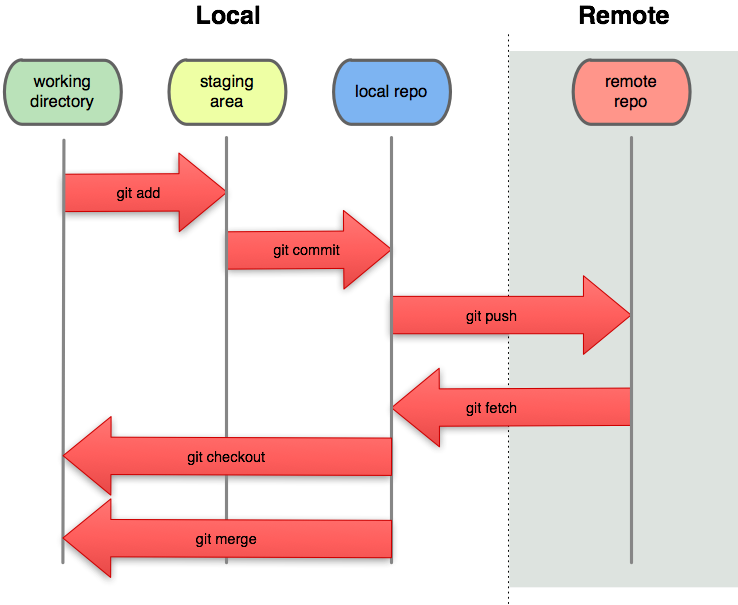
\includegraphics[scale=0.5]{local-remote.png}
     \end{center}
    \end{figure}
    \vfill
  \end{frame}

  \begin{frame}
    \frametitle{Área intermediária}
    \subsection{git}
    \begin{figure}[htb]
     \begin{center}
    	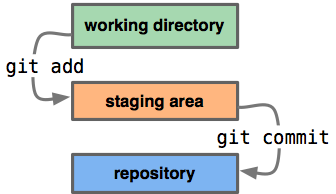
\includegraphics[scale=1]{index1.png}
     \end{center}
    \end{figure}
    \vfill
  \end{frame}

  \begin{frame}
    \frametitle{git é distribuido}
    \subsection{git}
    \begin{figure}[htb]
     \begin{center}
    	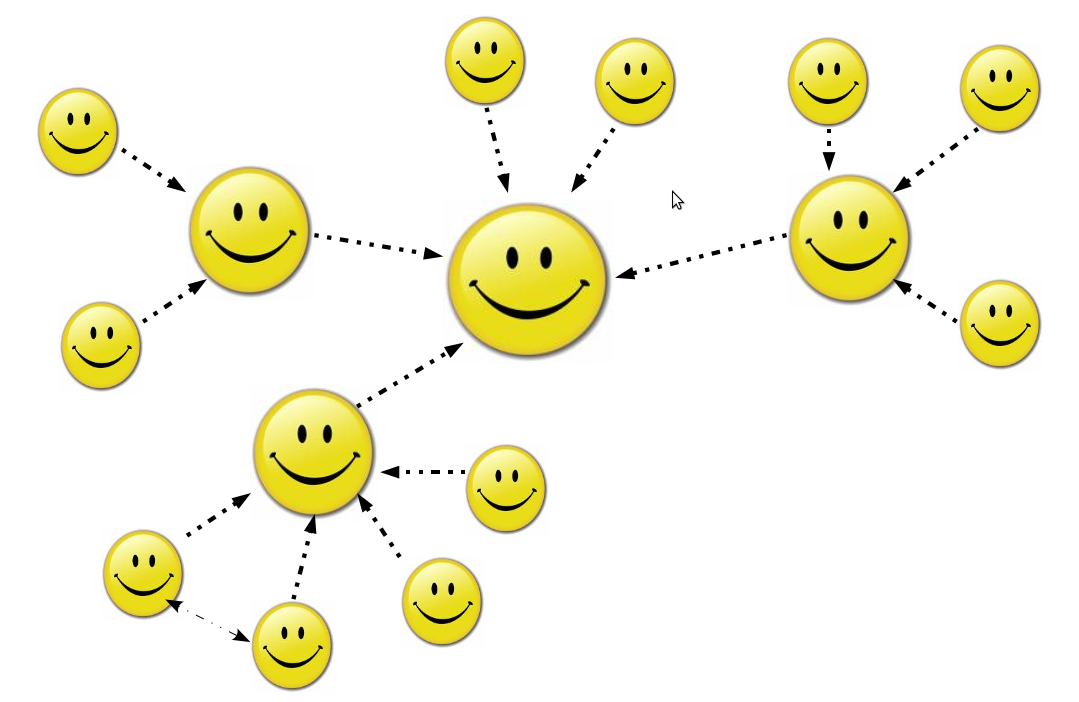
\includegraphics[scale=0.2]{descentralizado.png}
     \end{center}
    \end{figure}
    \vfill
  \end{frame}

  \section{Demonstração prática}
  \begin{frame}
    \frametitle{Uso do git}
    \vfill
      \begin{flushright}
        Juracy
    \end{flushright}
  \end{frame}

  \section{Ferramentas utilizadas}
  \begin{frame}
    \frametitle{Para este trabalho usamos:}
    \begin{itemize}
      \item Latex
      \item git e github
    \end{itemize}
  \end{frame}
  
    \section{Agradecimentos}
    \begin{frame}
        \frametitle{Agradecimentos}
        \begin{center}
            Obrigado !
        \end{center}
    \end{frame}

\end{document}

